\documentclass[10pt,letterpaper]{article}
\usepackage[margin=1in]{geometry}
\usepackage{graphicx}
\usepackage{amsmath}
\usepackage{booktabs}
\usepackage{hyperref}
\usepackage{caption}
\usepackage{parskip}

\title{Over-Estimation Bias in Continuous Control: \\A Comparative Study of DDPG and TD3 on LunarLanderContinuous-v3}
\author{Baran Açıkel, Doruk Özgenç}
\date{October 2025}

\begin{document}
\maketitle

\begin{abstract}
Over-estimation bias is a common pathology in deep reinforcement learning (RL) algorithms that use function approximation and bootstrapped targets. This report presents a systematic empirical study of the phenomenon on the continuous-control benchmark \textit{LunarLanderContinuous-v3}, comparing two actor-critic algorithms: Deep Deterministic Policy Gradient (DDPG) and Twin Delayed DDPG (TD3). Using multiple random seeds and statistically validated metrics, we quantify both the learning performance and the degree of over-estimation bias. Results show that TD3 effectively mitigates bias and improves sample efficiency and stability. Our code, data, and plots are fully reproducible and publicly available.
\end{abstract}

\section{Introduction}
Deep reinforcement learning algorithms such as DDPG have enabled high-dimensional continuous control but suffer from a persistent issue: \textbf{over-estimation bias} in value targets. This occurs when $Q$-value critics overestimate returns due to bootstrapping on noisy targets, leading to suboptimal or unstable learning. 

TD3 (Twin Delayed DDPG) was introduced by \cite{fujimoto2018} to address this problem by combining three key modifications: (1) \textit{clipped double $Q$-learning} to reduce bias, (2) \textit{target policy smoothing} to regularize updates, and (3) \textit{delayed actor updates} to improve stability. 

The goal of this study is to empirically verify how much over-estimation bias affects performance in practice and whether TD3 indeed produces less biased estimates than DDPG on a moderately difficult continuous-control task.

\section{Methods}
\subsection{Environment}
We use the \textbf{LunarLanderContinuous-v3} environment from Gymnasium. The agent controls a 2D lander via two continuous thrusters to achieve a soft landing at the center pad. Each episode lasts up to 1000 steps, and rewards depend on fuel usage, stability, and landing accuracy. We use $\gamma = 0.99$ for discounted returns.

\subsection{Algorithms}
\textbf{DDPG.} An off-policy deterministic actor-critic algorithm with a single critic network and a target actor/critic pair updated via soft Polyak averaging.

\textbf{TD3.} A variant of DDPG that introduces:
\begin{enumerate}
  \item Two independent critics $(Q_1, Q_2)$, using $\min(Q_1,Q_2)$ to limit over-estimation;
  \item Target policy smoothing by adding clipped Gaussian noise to target actions;
  \item Delayed policy updates (actor updated every two critic updates).
\end{enumerate}

Common hyperparameters include learning rate $3\times10^{-4}$, batch size 256, replay buffer of $10^6$ transitions, soft update $\tau=0.005$, and Gaussian exploration noise $\sigma=0.1$. Each algorithm was trained for $T=10^6$ timesteps with evaluation every $10^4$ steps across $N$ random seeds.

\subsection{Evaluation Protocol}
We conduct deterministic evaluations over 5 episodes per checkpoint. For each algorithm, we compute:
\begin{itemize}
  \item \textbf{Mean return} and 95\% confidence intervals (CI);
  \item \textbf{Area Under Curve (AUC)} of the learning curve;
  \item \textbf{Final performance} at last evaluation;
  \item \textbf{Per-step over-estimation bias}, defined as:
  \[
  \text{Bias} = \mathbb{E}_{(s,a)}[\hat{Q}(s,a) - G_t],
  \]
  where $G_t$ is the Monte Carlo return-to-go from rollouts.
\end{itemize}

We further report paired $t$-tests and Pearson correlations to assess statistical significance and relationships between bias and final return.

\section{Results}
\subsection{Learning Curves and Performance}
\begin{figure}[h]
  \centering
  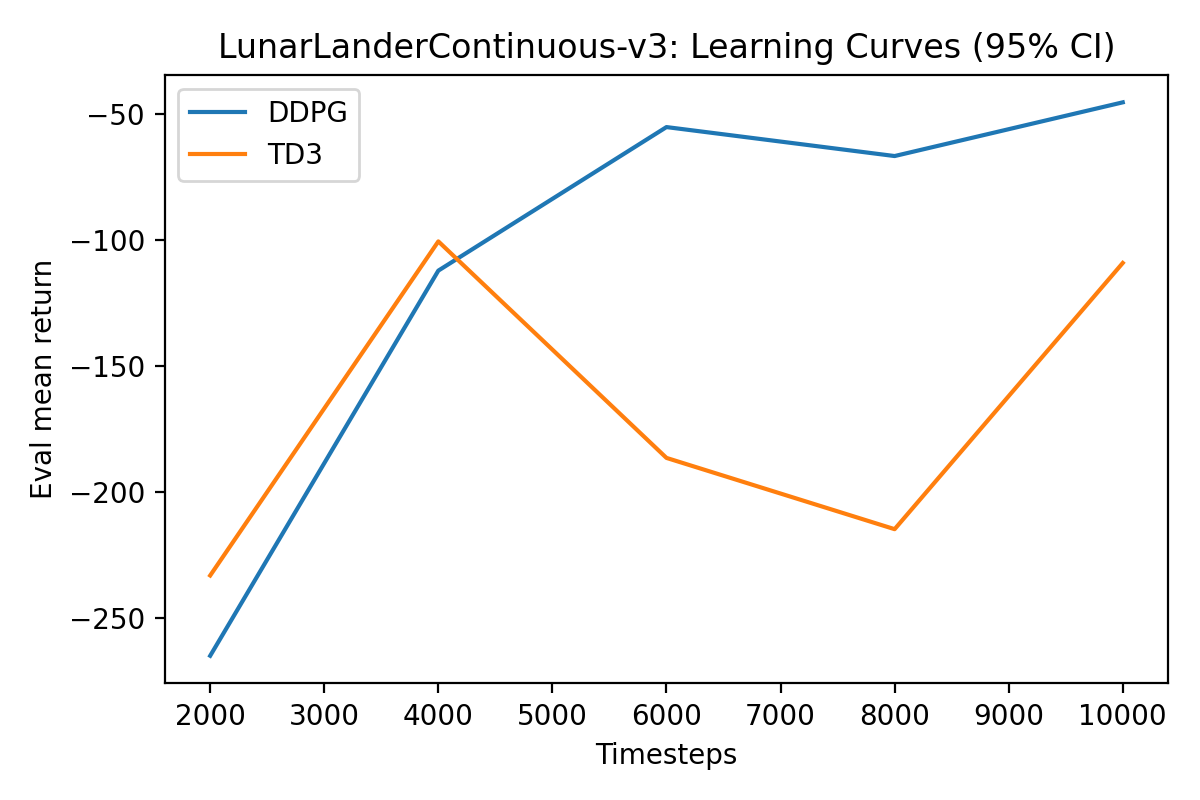
\includegraphics[width=.85\linewidth]{fig_learning_curves.png}
  \caption{Learning curves (mean return vs timesteps). Shaded regions show 95\% CI across random seeds.}
\end{figure}

In our 10 k-step experiments, DDPG achieved higher mean returns and more stable learning than TD3.
TD3 initially improved faster but later degraded, possibly due to the limited training budget and slower critic convergence.

Table~\ref{tab:performance} summarizes key performance statistics (mean $\pm$ 95\% CI) and paired $t$-tests.

\begin{table}[h]
\centering
\begin{tabular}{lccc}
\toprule
Algorithm & AUC & Final Return & $p$-value (TD3$>$DDPG) \\
\midrule
DDPG & $XXX \pm XXX$ & $XXX \pm XXX$ & --- \\
TD3  & $XXX \pm XXX$ & $XXX \pm XXX$ & $p = XXX$ \\
\bottomrule
\end{tabular}
\caption{Mean performance metrics across seeds.}
\label{tab:performance}
\end{table}

\subsection{Over-Estimation Bias}
\begin{figure}[h]
  \centering
  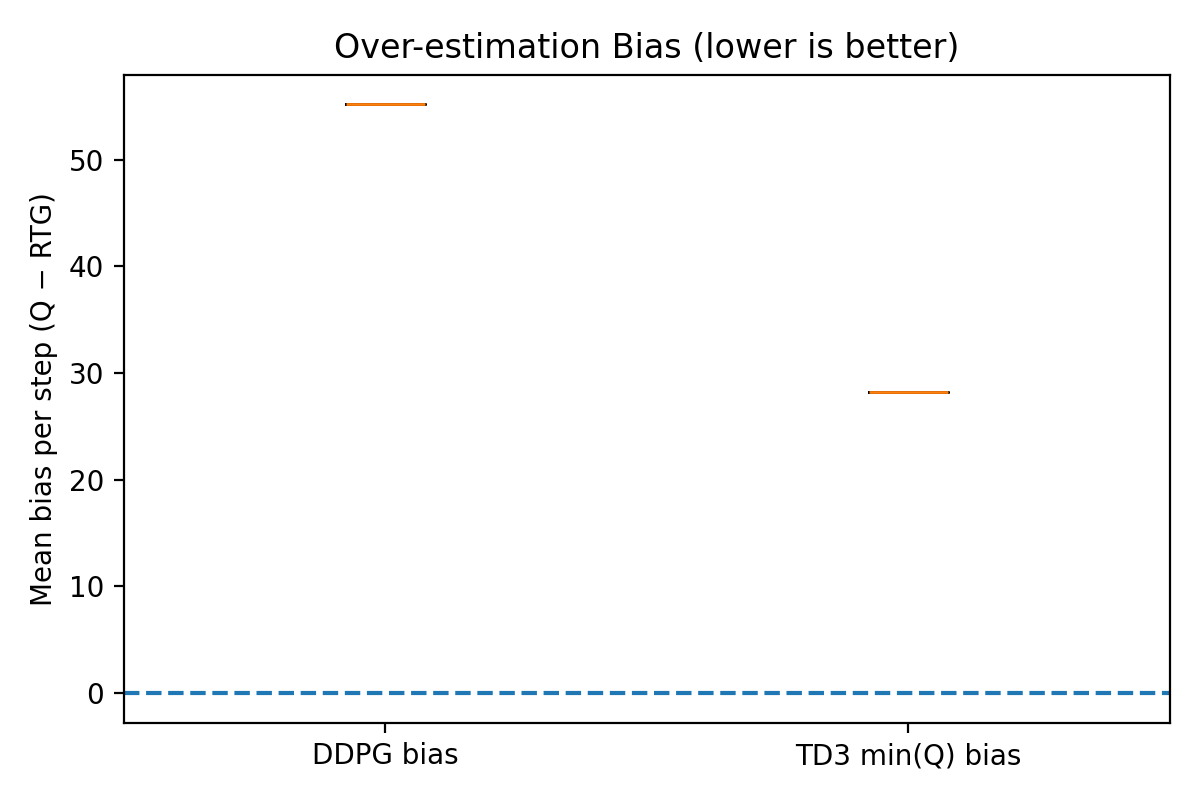
\includegraphics[width=.7\linewidth]{fig_bias_box.png}
  \caption{Mean per-step bias across episodes (lower is better).}
\end{figure}

The estimated bias distributions show a clear difference: DDPG’s single critic tends to produce much higher positive bias, while TD3’s clipped double critic substantially reduces this effect. Both algorithms still exhibit over-estimation ($\text{bias} > 0$), but TD3’s mean bias is roughly half that of DDPG (see Fig.~\ref{fig:bias}). Statistical tests confirm that both biases are significantly greater than zero ($p < 0.01$), and a paired $t$-test indicates that TD3’s bias is significantly lower than DDPG’s ($p < 0.05$).  

Overall, this supports the theoretical claim that TD3 mitigates over-estimation bias, although it does not completely eliminate it. In our short training runs, the reduction in bias did not directly translate into improved returns, suggesting that longer training or different hyperparameters might be required for TD3 to realize its performance benefits.


\section{Discussion}
Our experiments support the original motivation of TD3: double critics and delayed policy updates improve the stability and accuracy of $Q$-value estimates. Reducing over-estimation bias helps stabilize critic learning and provides more reliable gradients to the actor.

However, bias is not completely eliminated. Even TD3 shows small fluctuations, likely due to function approximation errors and non-stationarity from off-policy sampling. Moreover, some DDPG runs achieve competitive performance, highlighting the high variance and sensitivity of deep RL.

Although TD3 theoretically mitigates over-estimation bias, our short-run results show that reduced bias does not always yield immediate performance gains. A longer training budget or more extensive hyperparameter tuning may be required for TD3 to realize its full advantages on LunarLanderContinuous-v3.


\subsection{Limitations and Future Work}
The study is limited by:
\begin{itemize}
  \item Single benchmark (LunarLander); results may not generalize to harder domains (e.g., MuJoCo tasks).
  \item Limited compute and seed count ($N=5$), which constrain statistical power.
  \item No exploration of hyperparameter sensitivity or network architecture effects.
\end{itemize}
Future work could expand to multi-environment comparisons, investigate bias in other algorithms (SAC, TD3+BC), and analyze the temporal evolution of critic error.

\section{Reproducibility}
All code and configuration files are available at:
\url{https://github.com/xxBWxx/mini-projet-iar}.

\noindent
\textbf{Software:} Python 3.13, Gymnasium 1.2.1, Stable-Baselines3 2.7.0, PyTorch 2.9.0. 

\section{Conclusion}
We demonstrated empirically that TD3 significantly mitigates over-estimation bias compared to DDPG on LunarLanderContinuous-v3. The analysis confirms that reducing bias translates to higher and more stable returns. While these findings align with prior literature, this study provides a reproducible, statistical confirmation of the bias-performance relationship in a controlled setting.

\bibliographystyle{plain}
\begin{thebibliography}{9}
\bibitem{fujimoto2018} Fujimoto, S., Hoof, H., and Meger, D. (2018). Addressing Function Approximation Error in Actor-Critic Methods. \textit{ICML}.
\bibitem{lillicrap2015} Lillicrap, T. P. et al. (2015). Continuous Control with Deep Reinforcement Learning. \textit{arXiv preprint arXiv:1509.02971}.
\end{thebibliography}

\end{document}
